% !TeX root = main.tex

\chapter{Codierungstheorie}\label{chap:cod}

So schön die Aussagen von \cref{thm:channelCoding} sind, bleiben bei der praktischen Umsetzung einige Fragen und Probleme offen:
\begin{itemize}
  \item Die Aussage gilt für \enquote{sehr großes} $N$, in der Praxis muss die Blocklänge aber beherrschbar groß bleiben, damit die Latenz nicht zu groß wird: der Codierer eines $(N,K)$-Blockcodes kann einen Block erst verschicken, wenn $K$ Bits aus der Quelle gekommen sind. Das erste dieser $K$ Bits ist dann schon $K$ Takte \enquote{alt}, was \zB beim Telefonieren zu unerwünschten Verzögerungen führen kann. Außerdem führen größere Blocklängen generell zu komplexeren Algorithmen beim Decodieren.
  \item Die zufällige Codeerzeugung im Beweis von \cref{thm:channelCoding} ist nicht praktikabel. Erstens haben wir für einen gegebenen Code keine Möglichkeit herauszufinden, ob dieser wirklich gut genug oder zufällig schlecht ist. Außerdem ist es unmöglich, alle $2^K$ $N$-Wörter einzeln auszuwürfeln bzw.\ überhaupt nur aufzuschreiben. In der Praxis ist \zB $(N,K) = (1024, 512)$ eine übliche Größe. Ein solcher Code hat $2^{512}$ Codewörter mit jeweils \SI{1024}{\bit}. Um diesen Code aufzuschreiben, bräuchten wir $2^{512}⋅1024 = 2^{522}$ Nullen und Einsen (zum Vergleich: unser Universum hat geschätzt ungefähr $2^{240}$ Atome …).
  \item Der im Beweis verwendete Typische-Menge-Decodierer ist aus den gleichen Gründen hoffnungslos ineffizient: er müsste für ein empfangenes $y∈B^N$ \emph{jedes} der $2^K$ Codewörter $x∈\C$ durchgehen und ausrechnen ob $(x,y)∈T'_{N,β}$ gilt.
\end{itemize}
Deshalb werden Codes benötigt, deren Struktur man möglichst kompakt beschreiben und damit rechnen kann. In der Praxis werden heute fast ausschließlich \emph{lineare Codes} benutzt, die man bequem mit Matrizen darstellen kann und die wir in \cref{sec:linearCodes} behandeln. Vorher untersuchen wir noch einige allgemeine Eigenschaften von Codes, die deren Fehlerkorrekturfähigkeit bestimmen.

\begin{remark}
  Natürlich waren unsere Bemühungen in \cref{chap:IT} trotz der mangelnden Praktikabilität  nicht vergebens: immerhin wissen wir jetzt, bei welchen Codierungsraten wir überhaupt auf gute Fehlerkorrektur hoffen dürfen. Außerdem haben wir ein paar spannende Anschauungen und Resultate rund um die Entropie gewonnen und verstanden, was beim Zusammenfassen großer Datenblöcke passiert (Stichwort Typizität)!
\end{remark}

\begin{remark}
  In diesem Kapitel werden wir $\GF(2)^N$ als $N$-dimensionalen Vektorraum über dem Grundkörper $\GF(2)=\{0,1\}$ auffassen anstatt wie bisher nur als $N$-Tupel von Bits. Dies erlaubt uns, Elemente von $\GF(2)^N$ zu addieren, und Konzepte wie lineare Abhängigkeit, Dimension etc.\ aus der linearen Algebra zu verwenden. Zu beachten ist, dass in $\GF(2)$ wegen $1+1=0$ die Gleichung $1=-1$ gilt, weshalb in $\GF(2)^N$ Addition und Subtraktion identisch sind.
  
  In der Codierungstheorie ist es üblich, Vektoren als \emph{Zeilenvektoren}, also $1×N$-Matrizen zu definieren. Ist $w = w_1\dotsm w_N ∈ \GF(2)^N$, bezeichnet $w^T$ den entsprechenden Spaltenvektor, also eine $N×1$-Matrix.
\end{remark}


\section{ML-Decodierung und Codewort-Abstände}
Bei der Übertragung eines Codeworts über den BSC werden einige Bits vertauscht (von $0$ zu $1$ oder umgekehrt). Wenn dadurch das gesendete Codewort $x$ in ein anderes Codewort $x'≠x$ übergeht, hat der Decodierer keine Chance, diesen Fehler zu erkennen – er wird davon ausgehen, dass $x'$ gesendet und ohne Fehler übertragen wurde. Bei einem guten Code sollte also der \enquote{Abstand} zwischen zwei Codewörtern möglichst groß sein. Dazu definieren wir:


\begin{definition}[Hamming-Abstand]
  Sei $N∈ℕ$ und $x,y ∈ \GF(2)^N$. Dann heißt
  \[ \d(x,y) \coloneqq \abs{\{i\colon x_i ≠ y_i\}}\]
  der \emphex{Hamming-Abstand} von $x$ und $y$.
\end{definition}

\begin{lemma}\label{lem:hammingMetric}
  Der Hamming-Abstand definiert eine \emphex{Metrik} auf $\GF(2)^N$, \dh für $u,v,w \in \GF(2)^N$ gilt
  \begin{enumerate}
    \item \emph{Positive Definitheit:} $\d(u,v) ≥ 0$ und $\d(u,v) = 0$ genau für $u=v$,
    \item \emph{Symmetrie:} $\d(u,v) = \d(v, u)$
    \item \emph{Dreiecksungleichung:} $\d(u,v) ≤ \d(u,w) + \d(w,v)$ \label{lem:hamming-3}
  \end{enumerate}
  Außerdem ist er \emph{translationsinvariant}:
  \begin{enumerate}[resume]
    \item $\d(u+w, v+w) = \d(u,v)$. \label{lem:hamming-transInv}\hfill~
  \end{enumerate}
\end{lemma}
\begin{proof}
  Übungsaufgabe.
\end{proof}

Der im Beweis von \cref{thm:channelCoding} verwendete Typische-Menge-Decodierer ist nur für theoretische Zwecke interessant und in der Praxis weder realisierbar noch unbedingt sonderlich gut. Wir definieren nun stattdessen die \emph{Maximum-Likelihood-Decodierung}, die unter bestimmten Voraussetzungen \emph{optimal} für gegebenen Code und Kanal ist, also die kleinstmögliche Fehlerwahrscheinlichkeit erreicht.
%Die beste Decodierung erhalten wir offenbar, indem wir das (gegeben die Ausgabe $y$) am wahrscheinlichsten gesendete Codewort wählen, also
%\[\hat x = \argmax_{x∈\C} P(x∣y) = \argmax_{x∈\C} P(x\text{ gesendet}∣y\text{ empfangen})\tp\]
%Nach dem Satz von Bayes ist $P(x∣y) = P(y∣x)⋅P(x)/P(y)$, so dass
%\[ \hat x = \argmax_{x∈\C} \frac{P(y∣x)⋅P(x)}{P(y)}\]
%das gesuchte Codewort ist. Nehmen wir an, dass alle $x∈\C$ mit gleicher Wahrscheinlichkeit gesendet werden, ist der Term $P(x)$ konstant und kann deshalb beim maximieren weggelassen werden. Das $P(y)$ im Nenner hängt sowieso nicht von $x$ ab, so dass
%\[ \hat x = \argmax_{x∈\C} P(y∣x)\]
%ist, also das Codewort, das unter allen mit der größten Wahrscheinlichkeit zum beobachteten Output $y$ führt. Einen Ausdruck der Form $P(y∣x)$, bei denen $x$ als Variable angesehen wird, nennt man in der Statistik \emph{Likelihood-Funktion}, die eben hergeleitete Decodierstrategie entspricht dann einem \emph{Maximum-Likelihood (ML)-Schätzer}.
\begin{definition}
  Sei $\C$ ein $(N,K)$-Blockcode und $\K$ ein Kanal mit Ausgabealphabet $B$. Für $y∈B^N$ und $x∈\C$ bezeichne $P(y∣x) \coloneqq \prod_{i=1}^N P_{\K,x_i}(y_i)$ die Wahrscheinlichkeit, dass $y$ beim Empfänger ankommt, wenn $x$ gesendet wird. Ein Decodierer $D_{\ML}$, der für alle $y∈B^N$
  \[D_{\ML}(y) = \argmax_{x∈\C}P(y∣x)\]
  erfüllt, heißt \index{ML-Decodierer}\index{Maximum-Likelihood-Decodierer}\emph{Maximum-Likelihood (ML)-Decodierer}. Ein (nicht notwendigerweise eindeutiges) Codewort $\hat x$ mit $P(y∣\hat x) = \max_{x∈\C}P(y∣x)$ heißt \emph{ML-Codewort} für $y$.
\end{definition}
\begin{remark}
  Fasst man einen Ausdruck der Form $P(y∣x)$ als \emph{Funktion von $x$}, also der Bedingung auf, nennt man dies in der Statistik eine \emph{Likelihood-Funktion}. Wird eine Entscheidung basierend auf dem Maximum dieser Funktion getroffen, spricht man vom \emph{Maximum-Likelihood-Schätzer}.
  
  Der ML-Decodierer entscheidet sich für das Codewort $x$, welches unter allen am wahrscheinlichsten den Output $y$ hervorruft. In den Übungen werden Sie zeigen, dass 
  dies die optimale Strategie ist, wenn der Sender alle Codewörter mit gleicher Wahrscheinlichkeit verschickt.
  
  Leider ist die ML-Decodierung für fast alle Codes von praktischer Relevanz sehr schwer: es gibt keinen Algorithmus, der in vertretbarer Zeit ein ML-Codewort findet. Allerdings gibt es zahlreiche Decodieralgorithmen, die für spezielle Klassen von Codes zumindest recht nah an die Fehlerkorrekturrate eines ML-Decodierers kommen, diesen also \emph{approximieren}.
\end{remark}

Wir zeigen nun, dass beim BSC($ε$) ML-Codewörter gerade die mit kleinstem Hamming-Abstand zur Kanalausgabe $y$ sind.
\begin{lemma}\label{lem:MLdMin}
  Bei der Nachrichtenübertragung eines $(N,K)$-Blockcode $\C$ über den BSC($ε$) werde $x∈\C$ gesendet und $y∈\GF(2)^N$ empfangen. Dann gilt für $\hat x\coloneqq D_\ML(y)$:
  \[ \d(\hat x, y) = \min_{x∈\C}\d(x,y)\tk\]
  ein ML-Codewort hat also unter allen Codewörtern den kleinsten Hamming-Abstand zu $y$, und ein Decodierer, der zu jedem $y∈\GF(2)^N$ ein $x∈\C$ mit kleinstem Abstand findet, ist ein ML-Decodierer.
\end{lemma}
\begin{proof}
Für $\d(x,y)=l$ ($l$ Bits falsch und damit $N-l$ korrekt übertragen) gilt
\[P(y∣x) = \prod_{i=1}^N P_{\text{BSC}(ε),x_i}(y_i) = ε^l(1-ε)^{N-l}=\frac{ε^l (1-ε)^N}{(1-ε)^l} = \(\frac{ε}{1-ε}\)^l(1-ε)^N\tp\]
Wegen $ε<\frac12$ ist $\frac{ε}{1-ε} < 1$, so dass $P(y∣x)$ mit wachsendem $l$ streng monoton fällt, oder anders gesagt für kleinere $l$ größer ist. Um $P(y∣x)$ zu maximieren muss ein ML-Codewort $\hat x$ also $l$ minimieren: $\d(\hat x,y) = \min_{x∈\C}\d(x,y)$.
\end{proof}


Zur Vermeidung von Fehlern ist es nach \cref{lem:MLdMin} wünschenswert, dass zwischen je zwei Codewörtern möglichst viel Platz ist. Dazu definieren wir

\begin{definition} Sei $\C$ ein $(N,K)$-Blockcode. Wir nennen
  \[\d(\C) \coloneqq \min\{\d(x,x')\colon x,x'∈\C, x≠x'\}\]
  die \emphex{Minimaldistanz} von $\C$. Für den Fall $\abs{\C}=1$ legen wir $\d(\C) = 0$ fest.
\end{definition}

Für $x ∈ ℝ^3$ ist die Kugel um $x$ mit Radius $r>0$ definiert als die Menge aller Punkte $y$, die von $x$ höchstens den Abstand $\norm{x-y}_2 ≤ r$ haben. Mit dem Hamming-Abstand können wir äquivalent \enquote{Kugeln} im $\GF(2)^N$ definieren.
\begin{definition}
  Für $x ∈ \GF(2)^N$ und $r∈ℕ_0$ heißt
  \[ \B_r(x) = \{ y∈\GF(2)^N\colon \d(x,y) ≤ r\} \]
  die \emphex{Kugel} vom Radius $r$ um den Mittelpunkt $x∈\GF(2)^N$.
\end{definition}
\begin{remark}
  Für $x∈\GF(2)^N$ und $j∈ℕ_0$ ist $\abs{ \{ y\colon \d(x,y) = j\}} = \binom Nj$ (wähle $j$ der $N$ Einträge von $x$ aus, die geändert werden). Somit ist
  \[ \abs{\B_r(x)} = \sum_{j=0}^r \binom N j\tp\]
\end{remark}
\begin{theorem}
  Sei $\C$ ein Blockcode, $d\coloneqq \d(\C)$ und $t \coloneqq \left⌊\frac{d-1}2\right⌋$. Wird $x∈\C$ über den BSC($ε$) übertragen, $y∈\GF(2)^N$ empfangen und gilt $\d(x,y)≤ t$, folgt $D_\ML(y) = x$: die ML-Decodierung ist erfolgreich.
\end{theorem}
\begin{proof}
  Aus $t=⌊\frac{d-1}2⌋$ folgt $d≥2t+1$. Dann gilt
  \begin{equation}
    \B_t(x) ∩ \B_t(x')=∅
    \label{eq:disjointBalls}
  \end{equation}
  für alle $x,x'∈\C$ mit $x≠x'$: gäbe es nämlich ein $v∈\B_t(x)∩\B_t(x')$, erhalten wir mit der Dreiecksungleichung (\cref{lem:hammingMetric}, \cref{lem:hamming-3}) $2t+1 ≤ d ≤ \d(x,x') ≤ \d(x,v) + \d(v,x') ≤ t + t = 2t$, ein Widerspruch (siehe \cref{fig:balls} links). 
  \begin{figure}
    \centering
    \begin{tikzpicture}[scale=1.3]
      \draw (0,0) node[dot,"$x$" below] (x){} circle (1cm) edge ["$t$" above] ++(60:1cm);
      \draw (3,-.5) node[dot,"$x'$" below] (xx) {} circle (1cm) edge ["$t$" above] ++(60:1cm);
      \draw[brace] (x) -- node[above,sloped] {$≥d≥2t+1$} (xx);
      \node[dot,"$y$" left] at (-.5, .35) {};
    \end{tikzpicture}
    \quad
    \begin{tikzpicture}[scale=.75]
      \draw (0,0) node[dot,"$x$" below] (x){} circle (2.5cm) edge ["$d-1$" left] ++(60:2.5cm);
      \node[dot,"$x'$" below] (xx) at (3,-.5) {};
      \draw[brace] (x) -- node[above,sloped] {$≥d$} (xx);
      \node[dot,"$y$" left] at (2, -1) {};
    \end{tikzpicture}
    \caption{Links: disjunkte $t$-Kugeln um verschiedene Codewörter eines Codes $\C$ mit Minimaldistanz $\d(\C) ≥ 2t+1$. Fällt $y$ in $\B_t(x)$, kann es eindeutig decodiert werden. Rechts: Da $\B_{d-1}(x)$ außer $x$ keine Codewörter erkennt, wird ein Fehler erkannt, wenn $y$ in diese Kugel fällt.}\label{fig:balls}
  \end{figure}
  
  Gilt nun $\d(x,y)≤t$, kommt es also bei der Übertragung von $x$ zu höchstens $t$ Fehlern, gilt $y∈\B_t(x)$ und damit $y\notin \B_t(x')$ für alle $x≠x'\in \C$. Damit ist $x$ das eindeutige Codewort mit $d(x,y) =\min_{x'∈\C} \d(x',y)$, also nach \cref{lem:MLdMin} das eindeutige ML-Codewort, für das sich $D_\ML$ entscheiden muss.
\end{proof}

Bei mehr als $t$ Fehlern kann es passieren, dass der ML-Decodierer ein falsches Codewort ausgibt. Allerdings können wir eventuell immer noch \emph{erkennen}, dass es zu Übertragungsfehlern gekommen ist: Ist $\d(x,y)≤d-1$, so weiß der Decodierer, dass Fehler passiert sind, denn die Kugel $\B_{d-1}(x)$ enthält außer $x$ kein weiteres Codewort $x'∈\C$ (\cref{fig:balls} rechts). Man nennt einen Code mit Minimaldistanz $d$ deshalb auch \emph{$⌊(d-1)/2⌋$-fehlerkorrigierend} und \emph{$(d-1)$-fehlererkennend}.

\begin{example}\label{ex:correctingCodes}
  \begin{enumerate}
    \item Der $N$-Wiederholungscode $R_N = \{00\dotsm0, 11\dotsm1\} ⊆ \GF(2)^N$ hat die Minimaldistanz $\d(R_N) = N$ (es gibt nur $2$ Codewörter). Er kann somit (wie schon in \cref{ex:codingIntro} besprochen) $\frac{N-1}2$ Fehler korrigieren und $N-1$ erkennen.
    \item Der \emph{Kontrollcode} auf $\GF(2)^N$ ist definiert als
    \[\C \coloneqq \left\{ x = x_1\dotsm x_N ∈ \GF(2)^N\colon \sum_{i=1}^N x_i = 0\right\}\tk\]
    also die Menge aller $N$-Wörter mit sogenannter \emph{gerader Parität} (gerade Anzahl Einser). Seine Minimaldistanz ist $2$, so dass er keine Fehler korrigieren, aber einen erkennen kann.
    \item Der \emph{$(7,4)$-Hamming-Code}
        \[ \C \coloneqq \left\{ (x_1,\dotsc,x_7) ∈\GF(2)^7\colon \begin{aligned}
          \textcolor{red}{x_1 + x_2 + x_3 + x_5 }&\textcolor{red}{= 0} \\
          \textcolor{orange}{x_2 + x_3 + x_4 + x_6 }&\textcolor{orange}{= 0} \\
          \textcolor{blue}{x_1 + x_3 + x_4 + x_7}&\textcolor{blue}{= 0}\end{aligned} \right\} \]
    mit $N=7$, der in \cref{fig:hamming74} dargestellt ist, hat genau $2^4$ Codewörter: man kann nämlich jede der $2^4$ Belegungen von $x_1,\dotsc,x_4$ frei wählen, woraufhin dann die drei Gleichungen die Werte von $x_5, x_6, x_7$ festlegen; somit haben wir einen $(7,4)$-Code.
    \begin{figure}
      \centering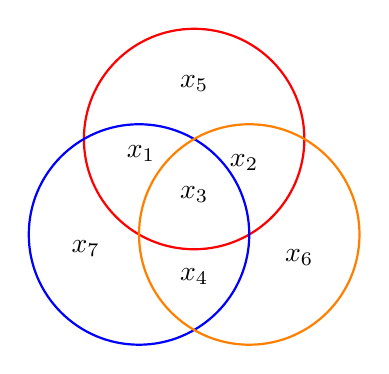
\begin{tikzpicture}[scale=.7]
        \draw[thick,draw=red] (0,0) circle (2cm)
          +(90:1cm) node {$x_5$}
          +(-90:1cm) node {$x_3$}
          +(-90:2.5cm) node {$x_4$}
          +(-25:1cm) node {$x_2$}
          +(-165:1cm) node {$x_1$};
        \draw[thick,draw=blue] (-120:2cm) circle (2cm)
          +(-165:1cm) node {$x_7$};
        \draw[thick,draw=orange] (-60:2cm) circle (2cm)
          +(-25:1cm) node {$x_6$};
      \end{tikzpicture}
      \quad
      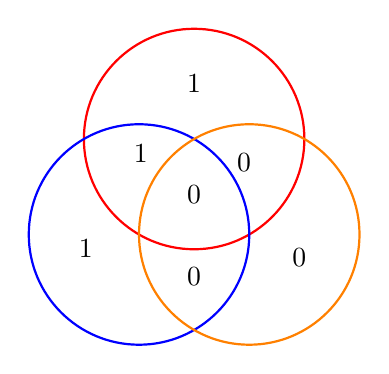
\begin{tikzpicture}[scale=.7]
          \draw[thick,draw=red] (0,0) circle (2cm)
            +(90:1cm) node {$1$}
            +(-90:1cm) node {$0$}
            +(-90:2.5cm) node {$0$}
            +(-25:1cm) node {$0$}
            +(-165:1cm) node {$1$};
          \draw[thick,draw=blue] (-120:2cm) circle (2cm)
            +(-165:1cm) node {$1$};
          \draw[thick,draw=orange] (-60:2cm) circle (2cm)
            +(-25:1cm) node {$0$};
      \end{tikzpicture}
      \quad
      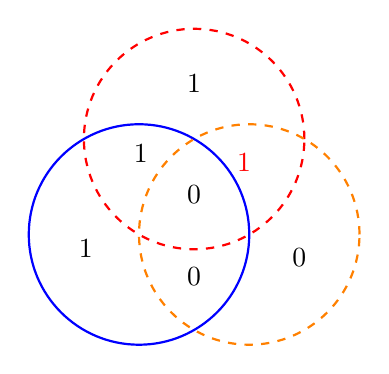
\begin{tikzpicture}[scale=.7]
          \draw[thick,draw=red,dashed] (0,0) circle (2cm)
            +(90:1cm) node {$1$}
            +(-90:1cm) node {$0$}
            +(-90:2.5cm) node {$0$}
            +(-25:1cm) node[text=red] {$1$}
            +(-165:1cm) node {$1$};
          \draw[thick,draw=blue] (-120:2cm) circle (2cm)
            +(-165:1cm) node {$1$};
          \draw[thick,draw=orange,dashed] (-60:2cm) circle (2cm)
            +(-25:1cm) node {$0$};
      \end{tikzpicture}
      \caption{\emph{Links:} Schematische Darstellung des $(7,4)$-Hamming-Codes aus \cref{ex:perfectCodes}. Die drei Kreise enstprechen den Teilmengen der Codewort-Einträge, die sich für die drei Bedingungen in der Definition des Codes zu $0$ aufsummieren müssen, in denen es also jeweils eine gerade Anzahl Einser geben muss. \emph{Mitte:} Beispielbelegung für das Codewort $x=1000101$. \emph{Rechts:} Bei einem Übertragungsfehler (hier in $x_2$) sind haben manche der Teilmengen (hier rot und orange) ungerade Parität. Es gibt genau eine Möglichkeit, durch Ändern eines einzigen Eintrags alle Paritäten wieder herzustellen.}
      \label{fig:hamming74}
    \end{figure}
    
    Dieser Code kann mit folgendem Verfahren einen Fehler korrigieren: berechne für jede der drei Teilmengen $I_1 = \{1,2,3,5\}$, $I_2 = \{2,3,4,6\}$, $I_3 = \{1,3,4,7\}$, die Parität $\sum_{i∈I_j} x_i$. Bei einem Übertragungsfehler muss mindestens eine Parität ungerade sein; je nachdem, wo der Fehler passiert ist, entweder eine (Fehler in $\{x_5, x_6, x_7\}$), zwei ($\{x_1, x_2, x_4\}$) oder alle drei (Fehler in $x_3$) der Summen $=1$. In jedem Fall gibt es genau eine Möglichkeit, durch Veränderung eines einzelnen Bits alle Paritäten wieder auf $0$ zu setzen. Also können wir einen Fehler korrigieren und erhalten $\d(\C)≥3$. Andererseits ist wegen $0000000, 1110000∈\C$ auch $\d(\C)≤3$, insgesamt also $\d(\C) = 3$.
  \end{enumerate}
\end{example}

Durch die disjunkten $t$-Kugeln wissen wir, das bei ML-Decodierung im Fall von höchstens $t$ Übertragungsfehlern korrekt decodiert wird. Bei mehr als $t$ Fehlern hängt dies jedoch von der genauen Struktur des Codes ab: entweder landet $y$ in der $t$-Kugel um ein falsches Codewort $x'$ (dann kommt es zum Decodierfehler) oder aber im Zwischenraum zwischen allen $t$-Kugeln – in diesem Fall könnte $x$ immer noch das Codewort mit kleinstem Abstand zu $y$ sein, muss aber nicht. Da dieser Fall schwer zu analysieren ist, wäre es schön, wenn es gar keinen solchen Zwischenraum gäbe – dann nennt man einen Code \emph{perfekt}.

\begin{definition}\label{def:perfect}
  Ein Code $\C$ mit Minimaldistanz $d≥1$ und $t=⌊(d-1)/2⌋$ heißt \emphex[Code!perfekter]{perfekt}, wenn 
  \[ \GF(2)^N = ⋃_{x∈\C} \B_t(x) \]
  gilt, die (disjunkte) Vereinigung aller $t$-Kugeln um die Codewörter also den ganzen Raum ausfüllt.
\end{definition}
Wir haben oben gezeigt dass die $t$-Kugeln um die Codewörter disjunkt sind, also überlappungsfrei im Raum $\GF(2)^N$ liegen. Da dort aber nur endlich viel Platz ist, können die Kugeln nicht beliebig groß werden, und es kann nicht beliebig viele geben. Die folgende Ungleichung präzisiert diesen Zusammenhang.

\begin{theorem}[Kugelpackungsschranke]\label{lem:spherePacking}
  Sei $\C$ ein $(N,K)$-Blockcode, $d=\d(\C)≥1$ und $t=⌊(d-1)/2⌋$. Dann gilt die \emphex{Kugelpackungsschranke} (auch \emphex{Hamming-Schranke} genannt)
  \[ 2^K \sum_{i=0}^t \binom Ni ≤ 2^N\tk\]
  die genau dann mit Gleichheit erfüllt ist, wenn $\C$ perfekt ist.
\end{theorem}
\begin{proof}
  Nach \cref{eq:disjointBalls} ist $\B_t(x) ∩ \B_t(x') = ∅$ für alle Codeworte $x≠x'$. Damit gilt
  \[ 2^N = \abs{\GF(2)^N} ≥ \abs{⋃_{x∈\C} \B_t(x)} = \sum_{x∈\C} \abs{\B_t(x)} = \sum_{x∈\C} \sum_{i=0}^t \binom Ni = \abs\C \sum_{i=0}^t\binom Ni = 2^K \sum_{i=0}^t \binom Ni\tp\]
  Die Gleichheit gilt nach \cref{def:perfect} genau für perfekte Codes.
\end{proof}

\begin{example}\label{ex:perfectCodes}
  \begin{enumerate}
    \item Der $3$-Wiederholungscode aus \cref{ex:codingIntro} und allgemein jeder $N$"=Wiederholungscode mit ungeradem $N=2t+1$ sind perfekt: es gibt nur die beiden Codewörter $0\dotsm0$ und $1\dotsm1$, und $\B_t(0\dotsm0)$ enthält alle $N$-Wörter mit mehr Einträgen $0$ als $1$, während $\B_t(1\dotsm1)$ genau den Rest enthält. 
    \item Für jedes $N$ ist der triviale Code $\C\coloneqq\GF(2)^N$ perfekt: seine Minimaldistanz ist $\d(\C)=1$, also $t=0$ und die $2^N$ \enquote{$0$-Kugeln} enthalten jeweils nur das Codewort selbst, überdecken also ganz $\GF(2)^N$.
    \item Der $(7,4)$-Hamming-Code aus \cref{ex:correctingCodes} ist nach \cref{lem:spherePacking} perfekt, denn mit $t=\frac{3-1}2=1$ gilt
            \[ 2^4 \sum_{i=0}^t \binom 7i = 16 (1 + 7) = 16⋅8 = 128 = 2^7 \tp\]
  \end{enumerate}
\end{example}
Wir werden im nächsten Abschnitt noch eine Klasse perfekter Hamming-Codes mit Minimaldistanz $d=3$ kennenlernen. Wir könnten nun darauf hoffen, die Aussage des Kanalcodierungssatzes (zumindest auf dem BSC($ε$)) mit perfekten Codes zu realisieren: wähle einen perfekten Code heraus, dessen Minimaldistanz $d$ groß genug ist, dass die Wahrscheinlichkeit von mehr als $t=⌊(d-1)/2⌋$ Übertragungsfehlern pro Codewort die gegebene Toleranz unterschreitet. Ein ML-Decodierer kann jedes empfangene $N$-Wort eindeutig decodieren, da es keinen Zwischenraum zwischen den $t$-Kugeln gibt. Leider ist dies nicht möglich:
\begin{theorem}
  Außer den trivialen Codes aus \cref{ex:perfectCodes} mit $t∈\{0,(N-1)/2\}$, den Hamming-Codes mit $t=1$ und einem $(23,12)$-Code mit $t=3$ existieren keine weiteren perfekten Codes.
\end{theorem}
Den Beweis dieses Satzes lassen wir aus. Anschaulich liegt das Problem darin, dass bei den meisten Codes der Zwischenraum zwischen den $t$-Kugeln den meisten Raum ausfüllt. Es ist einfach nicht möglich, diese Kugeln so anzuordnen, dass dazwischen kein Platz frei bleibt.


Neben der Kugelpackungsschranke gibt es eine weitere Ungleichung, die $N$, $K$ und $d$ eines Blockcodes in Beziehung setzt.
\begin{theorem}[Singleton-Schranke]\label{thm:singleton}
  Sei $\C$ ein $(N,K)$-Blockcode mit Minimaldistanz $\d(\C)=d$. Dann gilt die \emphex{Singleton-Schranke}
   \[d ≤ N-K+1.\]
 Erfüllt $\C$ diese Schranke mit Gleichheit, nennt man $\C$ einen \emphex{MDS-Code} (\emphex{maximum distance separable}).
\end{theorem}
\begin{proof}
  Sei
  \begin{align*}
    &π\colon \GF(2)^N → \GF(2)^{N-d+1}\\
    &π(x_1\dotsm x_N)=x_1\dotsm x_{N-d+1}
  \end{align*}
  die Projektion auf die ersten $N-d+1$ Komponenten. Da zwei verschiedene Codewörter von $\C$ sich in mindestens $d$ Stellen unterscheiden, können die ersten $N-d+1$ Stellen nicht gleich sein, so dass $π$ auf $\C$ injektiv ist und somit
  \[ 2^K = \abs\C = \abs{π(\C)} ≤ \abs{\GF(2)^{N-d+1}} = 2^{N-d+1}\]
  oder (nach Anwendung von $\log$ auf beiden Seiten) $K ≤ N-d+1$ bzw.\ $d≤N-K+1$ gilt.
\end{proof}
Der Begriff \emph{maximum distance separable} erklärt sich aus dem Beweis: bei MDS-Codes können wir die Projektion auf beliebige $K=N-d+1$ Koordinaten wählen und immer noch die verschiedenen Codewörter unterscheiden (\enquote{separieren}). Außer trivialen Beispielen gibt es keine binären MDS-Codes. Wir werden später aber mit den \emph{Reed-Solomon-Codes} eine Klasse von MDS-Codes über den Körpern $\GF(2^m)$ kennenlernen.

\section{Lineare Codes}\label{sec:linearCodes}
Im letzten Abschnitt haben wir uns mit den Abständen zwischen Codewörtern beschäftigt. Immer noch ungelöst ist allerdings das Problem, dass Codes praktischer Länge viel zu groß sein müssen, um alle Codewörter explizit aufzuschreiben. Der Ausweg besteht in \emph{linearen Codes}, die in so gut wie allen praktischen Anwendungen vorkommen; einer ihrer Vorteile ist, dass sie sich kompakt durch Matrizen darstellen lassen.

Obwohl wir mit linearen Blockcodes nur noch eine kleine Teilmenge \emph{aller} möglicher Codes betrachten, lässt sich zeigen, dass der Kanalcodierungssatz (\cref{thm:channelCoding}) auch für lineare Codes gilt; wir laufen also keine Gefahr, die \enquote{guten} Codes durch diese Einschränkung zu übersehen.

\begin{reminder}\label{rem:vectors}
  Sei $V$ ein Vektorraum über dem Körper $K$.
  \begin{enumerate}
     \item Eine Teilmenge $U⊆V$ heißt \emphex{Untervektorraum} oder einfach \emphex{Unterraum}, wenn $U$ selbst ein Vektorraum ist.
     \item $U⊆V$ ist genau dann Unterraum, wenn das \emphex{Unterraumkriterium} erfüllt ist, \dh für alle Vektoren $u,v∈U$ und alle Skalare $α∈K$ gilt
     \begin{itemize}
       \item $U≠∅$,
       \item $u+v∈U$,
       \item $αu∈U$.
     \end{itemize}
     \item Eine Teilmenge ${v_1,\dotsc,v_l}⊆V$ heißt \emphex{linear unabhängig}, wenn die Gleichung $\sum_{i=1}^l λ_i v_i = 0$ mit $λ_i∈K$ nur die eine Lösung $λ_1=\dotsm λ_l = 0$ hat.
     \item Eine Teilmenge $B=\{b_1,\dotsc,b_l\}⊆V$ heißt \emphex{Basis} von $V$, wenn $B$ linear unabhängig ist und $\left\{\sum_{i=1}^l λ_i b_i\colon λ_i∈K\right\} = V$ ist, $B$ also den ganzen Vektorraum $V$ aufspannt.
  \end{enumerate}
\end{reminder}
\begin{corollary}\label{lem:subspaceF2}
  Sei $V$ ein Vektorraum über dem Körper $\GF(2)$ und $0≠U⊆V$. $U$ ist genau dann ein Unterraum von $V$, wenn $u+v∈U$ für alle $u,v∈U$ gilt.
\end{corollary}
\begin{proof}
  Da es in $\GF(2)^N$ nur die zwei Skalare $0$ und $1$ gibt, ist Bedingung~3 des Unterraumkriteriums automatisch erfüllt: für alle $u$ gilt $0⋅u=2⋅u=u+u∈U$ nach Voraussetzung und $1⋅u=u∈U$ sowieso.
\end{proof}
\begin{definition}
  Ein $(N,K)$-Blockcode $\C$ heißt \emph{linear}\index{Code!linearer}, wenn $\C⊆\GF(2)^N$ ein Untervektorraum der Dimension $K$ ist.
  
  Eine Matrix $G∈\GF(2)^{K×N}$, deren Zeilen eine Basis von $\C$ bilden, heißt \emphex{Generatormatrix} für $\C$.
\end{definition}
\begin{remark}
  Ist $\C$ ein linearer $(N,K)$-Code und $G$ eine Generatormatrix von $\C$, gilt
    \[ \C = \{ w^T G\colon w ∈ \GF(2)^K \}\tp\]
  Damit können wir $G$ zum Codieren benutzen: die Abbildung
  \begin{align*}
    E_\C\colon &\GF(2)^K → \GF(2)^N\\
               &w → wG
  \end{align*}
  ist nach Voraussetzung (Zeilen von $G$ sind Basis, also linear unabhängig) injektiv und ihr Bild ist gerade der Unterraum $\C⊆\GF(2)^N$. Ein linearer $(N,K)$-Blockcode ist also durch die Angabe einer binären $K×N$-Matrix eindeutig bestimmt und kann mit $K⋅N$\,Bits abgespeichert werden. Im Vergleich zu den $2^K⋅N$\, Bits für allgemeine Codes (vgl.\ \cpageref{chap:cod}) ist dies eine drastische Reduktion; ein linearer $(1024,512)$-Code bräuchte so ungefähr \SI{512}{\kibi\byte}.
\end{remark}
\begin{example}
  Der $(7,4)$-Hamming-Code aus \cref{ex:correctingCodes} ist linear: für die drei dort definierten Teilmengen $I_1, I_2, I_3$ und $x^1, x^2 ∈ \C$ gilt nach Definition $\sum_{i∈I_j} x^k_i = 0$ für $k=1,2$ und $j=1,2,3$ und damit auch $\sum_{i∈I_j} (x^1 + x^2)_i = \sum_{i∈I_j} x^1_i + \sum_{i∈I_j} x^2_i = 0 + 0 = 0$ für $j=1,2,3$, so dass $x^1+x^2∈\C$ und $\C$ damit nach \cref{lem:subspaceF2} ein Unterraum von $\GF(2)^7$ ist.
  
  Wie in \cref{ex:correctingCodes} bemerkt, können die ersten vier Einträge jedes Codeworts frei gewählt werden, wodurch dann $x_5, x_6, x_7$ bestimmt sind. Wählen wir die vier Einheitsvektoren, erhalten wir eine Basis von $\C$ und damit die Generatormatrix
  \[ G = \begin{pmatrix} 1 & 0 & 0 & 0 & 1 & 0 & 1 \\
                         0 & 1 & 0 & 0 & 1 & 1 & 0 \\
                         0 & 0 & 1 & 0 & 1 & 1 & 1 \\
                         0 & 0 & 0 & 1 & 0 & 1 & 1\tp
         \end{pmatrix}\]
\end{example}

\begin{definition}
  Sei $N∈ℕ$. Für $x∈\GF(2)^N$ heißt
  \[\w(x) \coloneqq \d(x, 0) = \abs{\{i\colon x_i ≠ 0\}}\]
  das \emphex{Gewicht} von $x$. Für einen Code $\C$ heißt
  \[ \w(\C) \coloneqq \min_{0≠x∈\C} \{\w(x)\}\]
  das \emphex{Minimalgewicht} von $\C$. Für den Fall $\C ∖ \{0\} = ∅$ legen wir $\w(\C) = 0$ fest.
\end{definition}
\begin{lemma}\label{lem:dequalsw}
  Sei $\C$ ein linearer $(N,K)$-Code. Dann gilt $\d(\C) = \w(\C)$: die Minimaldistanz entspricht dem minimalen Gewicht eines Codeworts.
\end{lemma}
\begin{proof}
  Für $\abs\C=1$ muss $\C=\{0\}$ gelten, da $\C$ als Vektorraum die Null enthalten muss. Also ist $\w(\C) = 0$. Nach Definition ist für $\abs\C = 1$ auch $\d(\C)=0$, womit die Aussage gilt.
  
  Sei also $\abs\C>1$ und $x,x'∈\C$ mit $\d(x,x') = \d(\C)$. Dann gilt
  \[ \d(x,x') = \d(x-x',x'-x') = \d(x-x', 0) = \w(x-x')\]
  nach \cref{lem:hammingMetric}, \cref{lem:hamming-transInv}. Wegen der Linearität von $\C$ ist $x-x'∈\C$, also $\w(\C) ≤ \w(x-x') = \d(\C)$.
  
  Sei umgekehrt $x''∈\C$ mit $\w(x'') = \w(\C)$. Da $0∈\C$ gilt
  $\w(x'') = \d(x'', 0) ≥ \d(\C)$ und damit insgesamt $\w(\C) = \d(\C)$.
\end{proof}
\begin{remark}
  Auch wenn \cref{lem:dequalsw} die Bestimmung der Minimaldistanz etwas vereinfacht – statt $\d(x,y)$ für alle $\binom{\abs C}{2}$ Paare von zwei Codewörtern zu berechnen, müssen wir \enquote{nur} $\w(x)$ für alle $\abs \C = 2^K$ Codewörter berechnen – ist dies für die meisten Codes nicht praktikabel. Abgesehen von dem Fall, dass sich die Minimaldistanz eines Codes anhand seiner speziellen Struktur beweisen lässt (wie bei den Wiederholungscodes), gibt es keine effiziente Methode, $\d(\C)$ für einen beliebigen gegebenen (linearen) Code zu berechnen.
\end{remark}

Wir führen nun neben der Generatormatrix eine weitere Möglichkeit ein, einen linearen Code durch eine Matrix zu definieren.
\begin{definition}\label{def:parityCheck}
  Sei $\C ⊆ \GF(2)^N$ ein linearer $(N,K)$-Code. Eine Matrix $H∈\GF(2)^{(N-K)×N}$ heißt \emphex{Kontrollmatrix} für $\C$, wenn
  \[ \C = \{ x∈\GF(2)^N\colon Hx^T = 0 \} \]
  gilt.
\end{definition}
\begin{example}
  Die Kontrollmatrix des $(7,4)$-Hamming-Codes ergibt sich direkt aus dessen Definition, die ja gerade fordert, dass sich bestimmte Einträge eines Codeworts zu $0$ aufaddieren müssen: mit
  \[ H = \begin{pmatrix} 1 & 1 & 1 & 0 & 1 & 0 & 0 \\
                         0 & 1 & 1 & 1 & 0 & 1 & 0 \\
                         1 & 0 & 1 & 1 & 0 & 0 & 1 \end{pmatrix}\]
  haben wir
  \[ Hx^T = 0 ⇔ \begin{pmatrix}1\\0\\1\end{pmatrix} x_1 + \begin{pmatrix}1\\1\\0\end{pmatrix} x_2 + \dotsm + \begin{pmatrix}0\\0\\1\end{pmatrix} x_7 = 0⇔\begin{cases}
            x_1 + x_2 + x_3 + x_5 = 0 \\
            x_2 + x_3 + x_4 + x_6 = 0 \\
            x_1 + x_3 + x_4 + x_7= 0\end{cases}⇔ x∈\C \tp\]
\end{example}
\begin{lemma}
  Jeder lineare $(N,K)$-Code $\C$ besitzt eine Kontrollmatrix $H$.
\end{lemma}
\begin{proof}
  Für $x,y∈\GF(2)^N$ bezeichne $⟨x,y⟩ \coloneqq \sum_{i=1}^N x_iy_i$ das gewöhnliche Skalarprodukt. Dann ist das orthogonale Komplement zu $\C$,
  \[\C^⊥\coloneqq \{y∈\GF(2)^N\colon ⟨x,y⟩=0\text{ für alle }x∈\C\}\tk\]
  selbst ein Unterraum (und damit ein linearer Code), da offensichtlich $0∈\C^⊥$ und für $y, y'∈\C^⊥$ gilt $⟨x,y+y'⟩ = ⟨x,y⟩ + ⟨x,y'⟩ = 0+0 = 0$, also $y+y'∈\C^⊥$.
  
  Sei $H$ eine Generatormatrix für $\C^⊥$ mit Zeilen $h_1,\dotsc, h_m$ mit $m=\dim(\C^⊥)$. Wir zeigen, dass $H$ eine Kontrollmatrix für $\C$ ist, also dass $x∈\C ⇔ Hx^T = 0$ gilt.
  
  \enquote{$⇒$}: Ist $x∈\C$, gilt \[Hx^T =  \begin{pmatrix} ⟨h_1, x⟩\\\vdots \\ ⟨h_m, x⟩ \end{pmatrix} = \begin{pmatrix}0\\\vdots\\0\end{pmatrix}\tk\]
  da $h_i∈\C^⊥$ nach Definition.
  
  \enquote{$⇐$}: Ist umgekehrt $Hx^T = 0$, also $⟨h_i,x⟩=0$ für alle $i=1,\dotsc,m$. Jedes $y∈\C^⊥$ kann, da $h_1,\dotsc, h_m$ eine Basis von $\C^⊥$ ist, als $y=\sum_{i=1}^m λ_i h_i$ mit $λ_i∈\GF(2)$ geschrieben werden. Damit ist
  \[ ⟨y,x⟩ = \left⟨\sum_{i=1}^m λ_i h_i, x\right⟩ = \sum_{i=1}^m λ_i ⟨h_i, x⟩ = 0\]
  für alle $y∈\C^⊥$, also $x∈(\C^⊥)^⊥ = \C$ (die letzte Äquivalenz ist eine Übungsaufgabe). Damit erfüllt $H$ die Bedingungen in \cref{def:parityCheck}, ist also eine Kontrollmatrix für $\C$.
  
  Es bleibt zu zeigen, dass $m=N-K$ gilt, $H$ also $N-K$ Zeilen hat. Nach Definition ist $\C^⊥ = \op{Im}(H)$ und $\C=\op{Ker}(H)$; mt der Dimensionsformel folgt $N = \dim(\GF(2)^N) = \dim(\op{Im}(H)) + \dim(\op{Ker}(H)) = \dim(\C^⊥) + \dim(\C) = \dim(\C^⊥) + K$, also $\dim(\C^⊥) = N-K$ und damit $m=N-K$.
\end{proof}
\begin{remark}
  Auch wenn das Skalarprodukt $⟨⋅,⋅⟩$ auf $\GF(2)^N$ äquivalent zum euklidischen in $ℝ^N$ definiert ist, hat es auf endlichen Körpern andere Eigenschaften. Insbesondere gibt es Vektoren $0≠x∈\GF(2)^N$, die auf sich selbst orthogonal stehen, also $⟨x,x⟩=0$ erfüllen (\zB $x=(1,1)∈\GF(2)^2$), was im $ℝ^N$ unmöglich ist. Damit ist auch $\C^⊥$ kein Komplement im eigentlichen Sinne, da weder $\C∩\C^⊥=\{0\}$ noch $\C∪\C^⊥=\GF(2)^N$ garantiert sind. Es gibt sogar sogenannte \emph{selbstduale Codes} mit $\C^⊥=\C$, auf die wir hier jedoch nicht näher eingehen.
\end{remark}
Mit einer Kontrollmatrix können wir leicht überprüfen, ob ein $N$-Wort $y∈\GF(2)$ ein Codewort ist, indem wir die Bedingung $Hy^T=0$ überprüfen. Außerdem können wir Aussagen über die Minimaldistanz von $H$ ableiten. Die \emph{Hamming-Codes}, die wir gleich definieren, werden über ihre Kontrollmatrix definiert. An deren Struktur lässt sich ablesen, dass Hamming-Codes Minimaldistanz 3 haben, woraus wir dann ihre Perfektheit folgern werden.

\begin{definition}[Hamming-Codes]
  Zusätzlich zum bereits bekannten $(7,4)$-Hamming-Code definieren wir nun für jedes $m≥2$ einen Hamming-Code $\C$ mit $N=2^m-1$, $K=2^m-m-1$, und $\d(\C) = 3$ wie folgt: Sei $H$ eine $m×N$-Matrix, deren Spalten (in beliebiger Reihenfolge) alle Elemente von $\GF(2)^m∖\{0\}$ enthalten. Ein Code, dessen Kontrollmatrix $H$ ist, nennen wir \emph{Hamming-Code}.
\end{definition}
\begin{lemma}
  Sei $\C$ ein Hamming-Code zum Parameter $m≥2$.
  \begin{enumerate}
    \item $\d(\C) = 3$.
    \item $\C$ ist perfekt.
  \end{enumerate}
\end{lemma}
\begin{proof}
  \begin{enumerate}
    \item Seien $h_1,\dotsc, h_N$ die Spalten von $H$. Für $x∈\C$ gilt dann
    \[Hx^T = \sum_{i\colon x_i≠0} h_i = 0\]
    nach \cref{def:parityCheck}. Wir zeigen $\d(\C) = \w(\C)=3$ indem wir erst $\w(\C)∈\{1,2\}$ ausschließen und dann ein $x∈\C$ mit $\w(x) = 3$ konstruieren.
    
    Wäre $\w(\C)=1$, gäbe es ein $x∈\C$ mit $x_k=0$ für ein $k∈\{1,\dotsc,N\}$ und $x_i=0$ sonst. Dann wäre $0=Hx^T = h_k$, es gäbe also eine Nullspalte in $H$, was nach Definition von $H$ nicht stimmt. Wäre $\w(\C) = 2$, gäbe es $x∈\C$ und $k≠l$ mit
    \[x_i = \begin{cases} 1&i=k\text{ oder }i=l\tk,\\
                          0&\text{sonst.}
            \end{cases}\]
    und damit $0=Hx^T = h_k + h_l$, also $h_k = -h_l = h_l$ (da $1=-1$), es gäbe also zwei gleiche Spalten in $H$, was ebenso nicht stimmt.
    
    Seien nun $i_1, i_2, i_3$ die Spaltenindizes mit
    \[ h_{i_1} = \begin{pmatrix} 1\\0\\0\\\vdots\\0\end{pmatrix},
       h_{i_2} = \begin{pmatrix} 0\\1\\0\\\vdots\\0\end{pmatrix},
       h_{i_3} = \begin{pmatrix} 1\\1\\0\\\vdots\\0\end{pmatrix}\tk
    \]
    und $\hat x∈\GF(2)^N$ definiert durch
    \[ \hat x_i = \begin{cases} 1&i∈\{i_1,i_2,i_3\}\\ 0&\text{sonst.}\end{cases}\]
    so dass $Hx^T = h_{i_1} + h_{i_2} + h_{i_3} = 0$, also $\hat x∈\C$ gilt. Wegen $\w(\hat x) = 3$ gilt $\w(\C) ≤ \w(\hat x) = 3$, mit $\w(\C) > 2$ von oben also $\w(\C) = \d(\C) = 3$.
    \item Wir rechnen die Bedingung von \cref{lem:spherePacking} nach:
    \begin{align*}
      2^K \sum_{i=0}^1 \binom Ni &= 2^K\(\binom N0 + \binom N1\) \\
                             &= 2^{2^m-m-1} (1 + 2^m-1) \\
                             &= 2^{2^m-m-1} ⋅ 2^m = 2^{2^m-1} = 2^N\tp
    \end{align*}
  \end{enumerate}
\end{proof}

\section{Reed-Solomon-Codes}
\emph{Reed-Solomon-Codes} finden Anwendung in digitaler Fernseh- und Radioübertragung (DVB, DAB), auf Audio CDs oder QR-Codes. Auch wenn sie heutzutage langsam durch LDPC- und Turbo-Codes abgelöst werden, da für diese in den letzten Jahren besonders effiziente Decodieralgorithmen entwickelt wurden, gehören sie nach wie vor zu den wichtigsten und verbreitetsten Codes überhaupt. 

\begin{remark}
Für $n∈ℕ$ sei $\GF(2^n)$ der endliche Körper mit $2^n$ Elementen (siehe \cref{thm:finiteFields}) und $N∈ℕ$. Dann ist $\GF(2^n)^N$ wie bisher ein Vektorraum, nur dass die Einträge eines Vektors jetzt nicht mehr Bits aus $\GF(2)$, sondern Körperelemente von $\GF(2^n)$ sind.
\begin{enumerate}
  \item Ein linearer $(N,K)$-Blockcode über $\GF(2^n)$ ist ein linearer Unterraum von $\GF(2^n)^N$ der Dimension $K$.
  \item Der Hamming-Abstand von $x,y∈\GF(2^n)^N$ ist wie bisher definiert als
  \[\d(x,y) = \abs{\{i∈\{1,\dotsc, N\}\colon x_i ≠ y_i\}}\]
  nur dass jetzt $x_i,y_i∈\GF(2^n)$ sind. Genauso direkt verallgemeinern sich $\d(\C)$, $\w(\C)$ etc.
\end{enumerate}
Ist $\C$ ein linearer $(N,K)$-Blockcode über $\GF(2^n)$, erhalten wir einen (nicht notwendigerweise linearen) binären $(n⋅N, n⋅K)$-Blockcode $\tilde\C$, indem wir mit \cref{not:fieldVectorspace} jedes Element von $\GF(2^n)$ als $n$-Vektor über $\GF(2)$, also $n$ Bits, darstellen und diese aneinanderhängen. Wir können also auch mit nicht-binären Codes ohne große Umstände die Daten einer binären Quelle codieren und über einen binären Kanal verschicken.

Ist zum Beispiel $\C$ ein linearer $(3,2)$-Code über $\GF(2^4)$ und $x = (α_1,α_2,α_3)∈\C$, wobei  $α_i∈\GF(2^4)$ die Vektor-Darstellungen
\[ α_1 = (1, 1, 0, 1), α_2 = (0,0,1,0), α_3 = (0,1,1,0)\]
haben, so ist das entsprechende Codewort $\tilde x$ des entsprechenden $(4⋅3,4⋅2)$-Codes $\tilde\C$ über $\GF(2)$ gegeben durch $\tilde x = 110100100110$.

Warum tun wir uns den Umweg über $\GF(2^n)$ dann überhaupt an? Der Grund ist, dass man im nicht-binären Fall leichter \enquote{gute} Codes mit starken Eigenschaften (\zB hohe Minimaldistanz) findet – beispielsweise die gleich definierten Reed-Solomon-Codes.
\end{remark}

Wir benötigen noch ein Resultat aus der Algebra, das wir ohne Beweis zitieren:
\begin{theorem}
  Für jedes $n∈ℕ$ besitzt $\GF(2^n)^× = \GF(2^n) ∖ \{0\}$ einen \emphex{Erzeuger}, also ein Element $α∈\GF(2^n)$ mit
  \[ \left\{ α^0 (=1), α^1, α^2, \dotsc, α^{2^n-2} \right\} = \GF(2^n) ∖ \{0\}\tk\]
  wobei $α^k = \underbrace{α\dotsm α}_{k\text{-mal}}$. Außerdem gilt $β^{2^n-1}=1$ für alle $β∈\GF(2^n)^×$.
\end{theorem}
\begin{example}
  Mit $n=2$ erhalten wir den Körper $\GF(2^2)$ mit $4$ Elementen, die wir als Vektoren $(0,0)$, $(0,1)$, $(1,0)$, $(1,1)$ schreiben können, und nach \cref{not:fieldVectorspace} entspricht die Addition in $\GF(2^2)$ der Addition auf $\Z_2^2$, \zB $(0,1)+(1,1)=(1,0)$. Man kann zeigen, dass $α=(1,0)$ ein Erzeuger von $\GF(2^2)$ mit $α^0=(0,1)$ und $α^2=(1,1)$ ist. Dadurch ist dann auch die Multiplikation auf $\GF(2^2)$ bestimmt: sind $x=α^i,y=α^j∈\GF(2^2)^×$, gilt $x⋅y=α^{i+j}=α^{i+j\pmod{2^n-1}}$, \zB $(1,0)⋅(1,1) = α^1⋅α^2 = α^3 = α^0 = 1$. Für $x=(0,0)$ oder $y=(0,0)$ ist auch $x⋅y=0$, so dass wir alle Produkte haben (siehe \cref{tab:gf4}).
\end{example}
\begin{table}
  \centering
  \begin{tabular}{cc}
    \toprule
    Vektor & Potenz von $α$  \\
    \midrule
    $00$ & – \\
    $01$ & $α^0$ \\
    $10$ & $α^1$ \\
    $11$ & $α^2$ \\ \bottomrule
  \end{tabular}
  \qquad
  $\begin{array}{c|cccc}
  ⋅  & 00 & 01 & 10 & 11 \\ \hline
  00 & 00 & 00 & 00 & 00 \\ 
  01 & 00 & 01 & 10 & 11 \\
  10 & 00 & 10 & 11 & 01 \\
  11 & 00 & 11 & 01 & 10
  \end{array}$
  \caption{Der Körper $\GF(2^2)$. Links: Elemente in Vektordarstellung und als Potenz Erzeugers. Rechts: Multiplikationstabelle}
  \label{tab:gf4}
\end{table}

\begin{definition}[Polynome]
  Seien $n, K∈ℕ$ mit $K≤ 2^n$. Sei $\GF(2^n)[t]$ die Menge aller Polynome
  \[ f = a_r t^r + a_{r-1} t^{r-1} + \dotsm + a_1 t + a_0\]
  in der Variablen $t$ mit Koeffizienten $a_i ∈ \GF(2^n)$ (siehe \cref{def:polynom2}). Man kann zeigen, dass $\GF(2^n)[t]$ ein Vektorraum über dem Körper $\GF(2^n)$ ist. Sei
  \begin{align*}
    \GF(2^n)[t]_{K-1} &\coloneqq \{ f ∈ \GF(2^n)[t] \colon \deg f ≤ K-1 \}\\
    & = \left\{ a_{K-1} t^{K-1} + a_{K-2} t^{K-2} + \dotsm + a_1 t + a_0\colon a_i ∈\GF(2^n), i=0,\dotsc, K-1\right\}
  \end{align*}
  die Einschränkung auf Polynome vom Grad $\deg f ≤ K-1$.
\end{definition}

\begin{lemma}\label{ex:gf2ntk}
  $\GF(2^n)[t]_{K-1}$ ist ein $K$-dimensionaler Unterraum von $\GF(2^n)[t]$.
\end{lemma}

\begin{definition}[Reed-Solomon-Code]
  Seien $n, N,K∈ℕ$ mit $K≤N≤2^n$ gegeben. Sei $α$ ein Erzeuger von $\GF(2^n)^×$. Die Menge
  \[ \C \coloneqq \left\{ f(1), f(α), \dotsc, f\(α^{N-1}\)\colon f ∈ \GF(2^n)[t]_{K-1} \right\} ⊆ \GF(2^n)^N \]
  nennen wir den \emphex{Reed-Solomon-Code} RS($n,N,K$). Die Elemente von $\C$ entstehen also dadurch, dass wir irgendein Polynom $f∈\GF(2^n)[t]_{K-1}$ an den $N$ Stellen $1,α,\dotsc,α^{N-1}$ auswerten und die Ergebnisse zu einem $N$-Wort über $\GF(2^n)$ aneinanderhängen.
\end{definition}
\begin{remark}\label{rem:rsCoding}
  Aus der Definition von RS($n,N,K$) erhalten wir unmittelbar eine Codierungsfunktion $E_\C\colon \GF(2^n)^K → \GF(2^n)^N$: jedes $w = (w_1,\dotsc, w_K) ∈ \GF(2^n)^K$, können wir eindeutig mit einem Polynom $w(t) \coloneqq \sum_{i=0}^{K-1} w_{i+1} t^i ∈ \GF(2^n)[t]_{K-1}$ identifizieren (die $K$ Einträge von $w$ sind also die Koeffizienten des Polynoms) und dann $E_\C(w) = \(w(1),w(α),\dotsc,w\(α^{N-1}\)\)$ setzen.
\end{remark}
\begin{example}
  Sei $n=2$, $N=3$ und $K=2$. Dann ist $\GF(2^n)[t]_{K-1} = \GF(2^2)[t]_1$ die Menge aller Polynome vom Grad höchstens $1$:
  \[\GF(2^2)[t]_1  = \left\{ a_1 t + a_0\colon a_1, a_0 ∈ \GF(2^2) \right\}\tp\]
  Sei \zB $w=((1,0), (1,1)) = (α,α^2) ∈\GF(2^2)^K$. Dann ist $w(t) = α  + α^2⋅t ∈ \GF(2^2)[t]_1$ das entsprechende Polynom, und
  \begin{align*}
    E_\C(w) &= \( w(1), w(α), w(α^2) \) \\
            &= \( α + α^2⋅1, α+α^2⋅α, α + α^2⋅α^2 \)\\
            &= \( (1,0) + (1,1), (1,0) + (0,1), (1,0) + (1,0) \) \\
            &= \( (0, 1), (1,1), (0,0) \) = x∈ \GF(2^2)^N
  \end{align*}
  das Codewort zu $w$ mit der Binärdarstellung $x = 011100$.
\end{example}

\begin{lemma}\label{lem:rs}
  Seien $1≤K≤N≤2^n$ gegeben und $\C=$RS($n,N,K$) der entsprechende Reed-Solomon-Code. Dann ist $\C$ ein linearer $(N, K)$-Blockcode über $\GF(2^n)$ mit Minimaldistanz $\d(\C) = N-K+1$ und somit ein MDS-Code.
\end{lemma}
\begin{proof}
  Sei
  \begin{align*}
    φ&\colon \GF(2^n)[t]_{K-1} → \GF(2^n)^N\\
    f&↦ \(f(1),f(α),\dotsc, f\(α^{N-1}\)\)
  \end{align*}
  die \enquote{Auswertungsabbildung}, die ein Polynom an den Elementen $1,α,\dotsc,α^{N-1}$ auswertet.
  Diese Abbildung ist linear, da für $f_1, f_2 ∈ \GF(2^n)[t]_{K-1}$
  \begin{align*}
    φ(f_1 + f_2) &= \((f_1 +  f_2)(1),\dotsc, (f_1 + f_2)\(α^{N-1}\)\) \\
                   &= \(f_1(1) + f_2(1),\dotsc, f_1\(α^{N-1}\) + f_2\(α^{N-1}\)\) \\
                   &= φ(f_1) + φ(f_2)
  \end{align*}
  und analog $φ(λf_1) = λφ(f_1)$ für $λ∈\GF(2^n)$ gilt. Da $\C = φ(\GF(2^n)[t]_{K-1})$ das Bild von $\GF(2^n)[t]_{K-1}$ unter $φ$ ist und $\GF(2^n)[t]_{K-1}$ nach \cref{ex:gf2ntk} ein Unterraum ist, muss auch $\C$ ein Unterraum, also ein linearer Code sein. Wenn wir zeigen können dass $φ$ injektiv ist, haben wir dann nach der Dimensionsformel (Lineare Algebra) auch $\dim(\C) = \dim\(φ(\GF(2^n)[t]_{K-1})\) = \dim (\GF(2^n)[t]_{K-1}) = K$ nach \cref{ex:gf2ntk} gezeigt. Seien also $f,f'∈\GF(2^n)[t]_{K-1}$ mit
  \begin{align*}
    φ(f) = φ(f') &⇔ φ(f) - φ(f') = 0 \\
                  &⇔ \left(f(1) - f'(1), \dotsc, f\(α^{N-1}\) - f'\(a^{N-1}\)\right) = 0 \\
                  &⇔ \left((f-f')(1), \dotsc, (f-f')\(α^{N-1}\)\right) = 0 \\
                  &⇔ (f-f')(1) = \dotsm =  (f-f')\(α^{N-1}\) = 0\tk
  \end{align*}
  das Polynom $f-f'$ hat also $N$ verschiedene Nullstellen. Da aber $\deg(f-f') ≤ K-1$ und $K-1 < N$ nach Voraussetzung, impliziert dies nach \cref{cor:polyRoots} (ein von $0$ verschiedenes Polynom $f$ hat höchstens $\deg(f)$ Nullstellen) dass $f-f'=0$, also $f=f'$ und damit $φ$ injektiv, also auch $\dim(\C) = K$ ist.
  
  Es bleibt die Aussage über $\d(\C)$ zu zeigen. Da (wie wir eben schon verwendet haben) für jedes $0≠f∈\GF(2^n)[t]_{K-1}$ höchstens $K-1$ Einträge von $φ(f)$ Null sein können, müssen mindestens $N-(K-1)$ Einträge ungleich $0$ sein, woraus $\w(\C) ≥ \w(φ(f)) ≥ N-K+1$ folgt. Definieren wir andererseits
  \[\hat f(t) = \prod_{i=0}^{K-2} (t-α^i) ∈\GF(2^n)[t]_{K-1}\tk\]
  hat $\hat f$ die $K-1$ Nullstellen $1,α,\dotsc, α^{N-1}$, so dass nach demselben Argument wie oben $\hat f$ an den $N-K+1$ Stellen $α^{K-1},\dotsc,α^{N-1}$ nicht Null sein kann, also $\w(φ(\hat f)) = N-K+1$ und damit insgesamt $\w(\C) = N-K+1$ gilt. Da $\C$ die Singleton-Schranke (\cref{thm:singleton}) mit Gleichheit erfüllt, ist er ein MDS-Code.
\end{proof}
\section{Fallbeispiel: QR-Codes}
Ein \emphex{QR-Code} ist ein zweidimensionaler Barcode zur Repräsentation digitaler Daten, die in einer quadratischen Pixelmatrix als Schwarz-Weiß-Muster abgebildet werden, das zur automatischen Erfassung beispielsweise per Smartphone-Kamera geeignet ist, aber auch in der Produktionslogistik weite Verbreitung findet. Der ISO-Standard 18004 \cite{QR2005Standard} spezifiziert für verschiedene Datenmengen 40 Versionen in aufsteigender Größe ($21×21$ Pixel (Version 1) bis $177×177$ Pixel (Version 40)). Für jede Version stehen vier verschiedene Fehlerkorrektur-Levels L, M, Q, H zur Verfügung, die mittels Reed-Solomon-Codes die Korrektur von etwa 7\% (L) bis 30\% (H) Lesefehlern (beispielsweise bei Verschmutzung des Symbols oder schlechten Lichtverhältnissen beim Abfotografieren) erlauben.
\begin{Center}
\qrcode*{Dieser QR-Code enthält keinen sinnvollen Text.}
\end{Center}
Es stehen vier Datenmodi zur Verfügung, welche die effiziente Binärcodierung verschiedener Datentypen festlegen:
\begin{itemize}
  \item \emph{Numeric:} Dezimalzahlen, also Ziffernfolgen
  \item \emph{Alphanumeric:} Lateinische Großbuchstaben, Ziffern, einige Sonderzeichen
  \item \emph{Bytes:} beliebige Binärdaten, beispielsweise UTF-8-codierter Text mit deutschen Sonderzeichen; vgl. \cref{sec:AES}
  \item \emph{Kanji:} japanische/chinesische Zeichen
\end{itemize}
Die maximale Kapazität im jeweiligen Modus ist durch Version (Größe) und Fehler-Level bestimmt. Wir behandeln exemplarisch Version 6M ($41×41$ Pixel, ≈15\% Fehlerkorrektur) im \emph{Alphanumeric}-Modus, die bis zu 154 Zeichen aufnehmen kann, was für URLs, Kontaktdaten oder kurze Texte (ohne Sonderzeichen) ausreicht.
\subsection{Aufbau des QR-Codes}
Wir stellen den QR-Code als Matrix $Q∈\F_2^{41×41}$ dar, wobei eine $1$ für ein schwarzes, eine $0$ für ein weißes Pixel steht. Die Indizierung beginnt nach ISO-Standard bei $0$, so dass $Q_{0,0}$ die linke obere und $Q_{40,40}$ die rechte untere Ecke ist. Der vorhandene Platz von $41×41$ Pixeln ist in verschiedene Bereiche unterteilt (\cref{fig:qrcode}):
\begin{figure} \centering
  \begin{tikzpicture}[baseline,x=1mm,y=1mm,scale=1.3]
    \fill[LightGray] (0,0) rectangle (41, -41);
    \draw[step=1mm,very thin,gray] (0,0) grid (41, -41);
    \foreach \x/\y in {0/0, 34/0, 0/-34} {
      \begin{scope}[xshift=\x mm,yshift=\y mm]
      \fill[white]  (-1, 1) rectangle (8,-8); %separator
      \fill[Olive] (0,0) rectangle(7,-7);
      \fill[white] (1,-1) rectangle (6,-6);
      \fill[Olive] (2,-2) rectangle (5,-5);
      \end{scope}
    }
    \foreach \y in {0, -33}
      \fill[Teal] (8,\y) rectangle ++(1,-8);
    \foreach \x in {0, 33}
      \fill[Teal] (\x, -8) rectangle ++(8, -1);
    \foreach \i in {8,10,...,32} {
      \fill[DarkRed] (6,-\i) rectangle ++(1, -1);
      \fill[DarkRed] (\i, -6) rectangle ++(1, -1);
    }
    \foreach \i in {9,11,...,31} {
      \fill[white] (6,-\i) rectangle ++(1, -1);
      \fill[white] (\i, -6) rectangle ++(1, -1);
    }
    \fill[Teal] (8,-8) rectangle ++(1,-1);
    \fill[MediumSlateBlue] (32,-32) rectangle ++(5,-5);
    \fill[white] (33,-33) rectangle ++(3,-3);
    \fill[MediumSlateBlue] (34,-34) rectangle ++(1,-1);
    \draw[brace=mirror, font=\scriptsize] (0,-41.5) -- node[below] {$41$} (41,-41.5);
    \draw[brace=mirror, font=\scriptsize] (-.5, 0) -- node[left] {$7$} (-.5, -7);
    \draw[brace=mirror, font=\scriptsize] (-.5, -8) -- node[left] {$25$} (-.5, -33);
    \draw[brace, font=\scriptsize] (41.5, 0) -- node[right] {$41$} (41.5, -41);
    \end{tikzpicture}
  \caption{Aufbau eines QR-Codes Version 6M. \textcolor{Olive}{Positionsmuster (incl. Trennstreifen)} und \textcolor{MediumSlateBlue}{Ausrichtungsmuster} sowie \textcolor{DarkRed}{Synchronisationsmuster} sind fest. Die \textcolor{Teal}{Format-Information} speichert Fehlerlevel (hier: M) und Maske in codierter Form. Der übrige Platz wird für die RS-codierten Nutzdaten verwendet.}
  \label{fig:qrcode}
\end{figure}
\begin{enumerate}
  \item Immer gleiche \emph{Positionierungs-Muster} enthalten keine Information, sondern helfen den Bilderkennungs-Algorithmen beim korrekten Auffinden des QR-Codes in einem Foto. Es gibt:
  \begin{itemize}
    \item Drei $7×7$-\textcolor{Olive}{Positions-Muster} aus konzentrischen Quadraten mit den Mittelpunkten $Q_{3,3}$, $Q_{37,3}$, $Q_{3,37}$ erlauben das Finden des QR-Codes im Foto; da es in der rechten unteren Ecke fehlt, kann Rotation erkannt werden. Nach innen sind die Muster jeweils durch 1 Pixel breite weiße Trenner abgegrenzt.
    \item Ein $5×5$-\textcolor{MediumSlateBlue}{Ausrichtungs-Muster} mit Mittelpunkt bei $Q_{34,34}$ (größere QR-Code-Versionen enthalten mehr davon).
    \item \textcolor{DarkRed}{Synchronisations-Muster}: je eine Zeile bzw. Spalte abwechselnd $1/0$-Pixel in Spalte und Zeile $6$ zwischen den Positions-Mustern. Erleichtert die Synchronisation zwischen Bild-Koordinaten und Matrix-Indizes bei Verzerrung (\zB schräge Aufnahme).
  \end{itemize}
  Zusätzlich sollte der gesamte QR-Code mit einer mindestens 4 Pixel breiten weißen Randzone umgeben sein.
  \item \textcolor{Teal}{Format-Information}: Meta-Information über verwendete Fehlerkorrektur und \emph{Maske} (siehe später), inkl.\ Fehlerkorrektur.
  \item Die eigentlichen Nutzdaten, die zunächst binär codiert und dann mit einem Reed-Solomon-Code über $\GF(2^8)$ gegen Fehler abgesichert werden.
\end{enumerate}
Von den $41^2$ Pixeln sind $3⋅\textcolor{Olive}{8^2} + \textcolor{MediumSlateBlue}{5^2} + 2⋅\textcolor{DarkRed}{25} + \textcolor{Teal}{31}$ \enquote{besetzt}, für die codierten Nutzdaten bleiben somit \SI{1383}{\bit} übrig.

\subsection{Quellencodierung: von Zeichen zu Bits}
Im alphanumerischen Modus stehen 45 verschiedene Zeichen zur Verfügung, die wir nach \cref{tab:alphanum} mit dem Alphabet $A= \{0,\dotsc,44\}$ identifizieren.
\begin{table}
  \begin{tabular}{r|ccccccccccccccccc}\toprule
  Zeichen: & 0 & …  & 9 & A & B & … & Z & \emph{Leerz.} & \$ & \% & * & + & - & . & / & : \\
  Wert: & 0 & … & 9 & 10 & 11 & … & 35 & 36 & 37 & 38 & 39 & 40 & 41 & 42 & 43 & 44 \\ \bottomrule
  \end{tabular}
  \caption{Zuordnung der erlaubten alphanumerischen Zeichen zu einem Zahlwert zwischen $0$ und $44$.}
  \label{tab:alphanum}
\end{table}
Die zu speichernde Information können wir daher als Wort
 \[w = w_1w_2\dotsm w_k ∈ A^k\]
mit $k \coloneqq l(w) ≤ 154$ Zeichen darstellen. Sei
$\op{bin}_{s}(x)\colon \{0,\dotsc,2^s-1\} → \GF(2)^s$ die Darstellung  einer natürlichen Zahl als $s$ Bit lange Binärzahl (\zB $\op{bin}_5(6) = 00101$). Die $fw_i$ werden nun zu $⌊k/2⌋$ Paaren aus jeweils zwei Zahlen zusammengefasst:
\[ w = ((w_1, w_2), (w_3, w_4), \dotsc)\tk\]
wobei für $l$ ungerade am Ende noch $w_k$ einzeln übrig bleibt. Diese Paare werden nun mit der injektiven Abbildung
\begin{align*}
  E_Q\colon A×A &→ \GF(2)^{11} \\
   (z_1, z_2) &↦ \op{bin}_{11}(45⋅z_1 + z_2)
\end{align*}
binär codiert und die Ergebnisse aneinandergehängt. Ist $k$ ungerade, wird das letzte Zeichen $w_k$ zu einer $6$-Bit-Zahl $\op{bin}_6(w_k)$.
\begin{remark}
  Ganz im Sinne von \cref{thm:sourceStrong} codieren wir paarweise, um weniger Kapazität zu verschwenden: zur einzelnen Codierung eines $a∈A$ bräuchten wir $6$ Bits, da $\abs A = 45 > 2^5 = 32$, mit $5$ Bits geht es also nicht. Andererseits können wir Paare $(a,b)∈A^2$ mit $11$ Bits codieren, da $\abs{A^2} = 45^2 = 2025 < 2^{11} = 2048$. Der Unterschied $2048/2025$ ist so klein, dass es sich nicht lohnt, noch mehr Zeichen zusammenzufassen.
\end{remark}
Der so berechneten Binärfolge wird noch das feste 4-Tupel $0010$, das den alphanumerischen Modus ankündigt, sowie der \emphex{Zeichenzähler} $\op{bin}_9(k)$ (damit der Empfänger später weiß, wie lang die eigentliche Nachricht ist) vorangestellt und die \emphex{Endmarke} $0000$ angehängt; insgesamt erhalten wir die binäre Nachricht
\[ m(w) = \underbrace{0010}_{\text{Modus}}\; \underbrace{\op{bin}_9(k)}_{\text{Zeichenzähler}}\; \underbrace{E_Q(w_1, w_2)\; E_Q(w_3, w_4) \dotsm [\op{bin}_6(w_k)]}_{\text{Daten}}\; \underbrace{0000}_{\text{Endmarke}}\tk\]
wobei $\op{bin}_6(w_k)$ nur für ungerade $k$ vorkommt. Da $k≤154$ ist die Bitlänge maximal $l(m(w)) ≤ 4 + 9 + (154/2)⋅11 + 4 = 864$.
\begin{example}
  Die Nachricht \t{AC-42} soll codiert werden. Laut \cref{tab:alphanum} entspricht dies der Zahlenfolge $w = (10,12,41,4,2)$, $k= l(w) =5$. Wir erhalten die Paare $(10,12)$, $(41,4)$ und den Rest $(2)$, und somit $E_Q(10,12) = \op{bin}_{11}(45⋅10+12) = \op{bin}_{11}(462) = 00111001110$, $E_Q(41,4) = 11100111001$ und $\op{bin}_6(2) = 000010$. Da $k=5$, ist der Zeichenzähler $\op{bin}_9(5) = 000000101$ und die gesamte Nachricht somit
  \[ m(\t{AC-42}) = 0010 000000101 00111001110 11100111001 000010 0000\tp\]
\end{example}
\subsection{Umrechnung in Bytes}
Um einen RS-Code über $\GF(2^8)$ zu verwenden, wird die im letzten Abschnitt erzeugte binäre Nachricht $m(w)$ in \emph{Bytes}, also Blöcke von jeweils \SI{8}{\bit} unterteilt. Falls $8 \nmid l(m(w))$, werden dazu weitere $0$er an $m(w)$ angehängt, bis die Länge ein Vielfaches von $8$ ist. Wir erhalten somit ein \enquote{Byte-Wort} $b(m) = b_1,\dotsc, b_n$, $b_i ∈ \GF(2)^8$. Ein QR-Code Version 6M kann insgesamt \num{108} Bytes an Nutzdaten aufnehmen. Ist $n < 108$, werden zum Auffüllen abwechselnd die festen Bytes $11101100$ und $00010001$ angehängt, so dass am Ende genau \num{108} Bytes $b = b_1, \dotsc, b_{108}$ an Nutzdaten vorliegen.

\subsection{Reed-Solomon-Codierung}
\begin{theorem}\label{thm:rsCoding2}
  Sei $1≤K≤N≤2^n$, $α$ ein Erzeuger von $\GF(2^n)$ und $g(t) \coloneqq \prod_{i=0}^{N-K}(t-α^i)$. Für $w=(w_1,\dotsc, w_K) ∈\GF(2^n)^K$ sei wie in \cref{rem:rsCoding} $w(t) = \sum_{i=0}^{K-1} w_{i+1} t^i$ und $r^w(t)$ der Rest bei Polynomdivision von $t^{N-K}⋅w(t)$ durch $g(t)$, also $t^{N-K}⋅w(t) = g(t)⋅q(t) + r^w(t)$ für ein Polynom $q(t)$ und $\deg(r^w(t)) < \deg(g(t)) = N-K$. Dann ist
  \begin{align*}
    E_\C\colon \GF(2^n)^K &→ \GF(2^n)^N \\
                        w &↦ \(w_1, \dotsc, w_k, r^w_1,\dotsc, r^w_{N-K}\)
  \end{align*}
  eine Codierungsfunktion für RS($n,N,K$).
\end{theorem}
Im Gegensatz zu \cref{rem:rsCoding} müssen wir also nur \emph{eine} Polynomdivision ausführen und dann die Koeffizienten des Restpolynoms an die Eingabe $w$ anhängen, um das Wort $w$ mit einem Reed-Solomon-Code zu codieren. Eine Codierungsfunktion $E_\C$ der Form $E_\C(w) = (w, f(w))$, bei der jedes Codewort in den ersten $K$ Komponenten gerade der Eingabe entspricht, nennt man \emphex{systematisch}.

Die 108 Byte $b = b_1\dotsm b_{108}$ aus dem vorigen Abschnitt werden jetzt in vier Gruppen $\tilde b_1, \dotsc, \tilde b_4$ zu je 27 Byte zusammengefasst ($27⋅4=108$). Nach \cref{not:fieldVectorspace} fassen wir jedes $\tilde b_i$ als Element von $\GF(2^8)^{27}$ auf, das nach der Methode aus \cref{thm:rsCoding2} mit dem RS($8, 43, 27$)-Code zu einem Codewort $c_i = (\tilde b^i, \tilde r^i) ∈ \GF(2^n)^43$ mit $\tilde r^i ∈ \GF(2^n)^{16}$ codiert wird. Nach \cref{lem:rs} hat dieser Code die Minimaldistanz $43-27+1 = 17$ und kann so auf dem BSC bis zu $(d-1)/2 = 8$ Fehler oder $8/43 ≈ \SI{18.6}{\percent}$ korrigieren. Die vier Codewörter $c^1,\dotsc,c^4$ können damit insgesamt bis zu \num{32} Fehler korrigieren – aber nur, wenn sich diese \enquote{gleichmäßig} verteilen, so dass in jedem Codewort genau $8$ Fehler passieren. Landen hingegen alle Fehler im selben Codewort, reichen schon $9$ Fehler (und damit $9/143≈\SI{6.3}{\percent}$) für einen Decodierfehler. 

\subsection{Verteilung der Bytes in $Q$}
Um zu vermeiden, dass alle Fehler im selben Codewort vorkommen, werden die Daten der vier Codewörter $c^1,\dotsc,c^4$ vor der Platzierung in der Matrix $Q$ \enquote{durcheinandergewürfelt}. Die Idee ist, dass Fehler beispielsweise durch Flecken oder Verdeckung eines Teils des QR-Codes oft auf einem kleinen Bereich der Matrix gehäuft auftreten. Das Durcheinanderwürfeln sorgt dann dafür, dass die Codewörter trotzdem etwa gleichmäßig von diesen Fehlern betroffen sind. Sei $\tilde b^i = (b^i_1, \dotsc, b^i_{27})$ und $r^i = (r^i_1,\dotsc,r^i_{16})$. Die endgültige Byte-Sequenz $x ∈ \GF(2^8)^{172}$ erhalten wir nach der Vorschrift
\[ x = b^1_1 \dotsm b^4_1 \dotsm b^1_{27} \dotsm b^4_{27} r^1_1 \dotsm r^4_1 \dotsm r^1_{16} \dotsm r^4_{16}\ts\]
die Einträge der folgenden Tabelle werden also spaltenweise von oben nach unten und von links nach rechts aneinandergehängt.
\[ \begin{array}{cccc|cccc} \toprule
     \multicolumn{4}{c}{\tilde b^i} & \multicolumn{4}{c}{r^i} \\ \midrule
 b^1_1 & b^1_2 & \dots & b^1_{27} & r^1_1 & r^1_2 & \dots &r^1_{16} \\
 b^2_1 & b^2_2 & \dots & b^2_{27} & r^2_1 & r^2_2 & \dots &r^2_{16} \\
 b^3_1 & b^3_2 & \dots & b^3_{27} & r^3_1 & r^3_2 & \dots &r^3_{16} \\
 b^4_1 & b^4_2 & \dots & b^4_{27} & r^4_1 & r^4_2 & \dots &r^4_{16} \\\bottomrule
 \end{array}
\]
Nun ist jedes $x_i$, $1≤i≤172$, ein Element von $\GF(2^8)$, das wir wieder nach \cref{not:fieldVectorspace} als Byte $x_{i,1},\dotsc, x_{i,8}$, also \SI{8}{\bit} aus $\GF(2)^8$ schreiben. Die $172$ Bytes werden nun zweispaltig schlangenförmig von unten rechts nach oben links in der Matrix $Q$ verteilt, wobei Einträge, die durch Positionsmuster etc.\ schon belegt sind, einfach übersprungen werden. Ein $x_i∈\GF(2^8)$ belegt so in der Regel eine $2×4$-Teilmatrix von $Q$ (siehe \cref{fig:bitPlacement}).

\begin{figure}
  \centering
  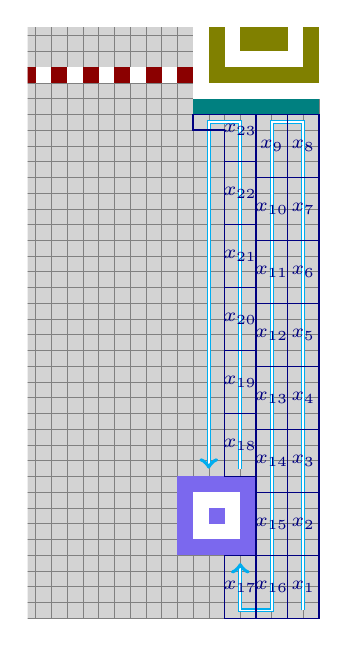
\begin{tikzpicture}[x=1mm,y=1mm,scale=2,font=\scriptsize]
      \path[clip] (22.5, -3.5) rectangle (42,-42);
      \fill[LightGray] (0,0) rectangle (41, -41);
      \draw[step=1mm,very thin,gray] (0,0) grid (41, -41);
      \foreach \x/\y in {0/0, 34/0, 0/-34} {
        \begin{scope}[xshift=\x mm,yshift=\y mm]
        \fill[white]  (-1, 1) rectangle (8,-8); %separator
        \fill[Olive] (0,0) rectangle(7,-7);
        \fill[white] (1,-1) rectangle (6,-6);
        \fill[Olive] (2,-2) rectangle (5,-5);
        \end{scope}
      }
      \foreach \y in {0, -33}
        \fill[Teal] (8,\y) rectangle ++(1,-8);
      \foreach \x in {0, 33}
        \fill[Teal] (\x, -8) rectangle ++(8, -1);
      \foreach \i in {8,10,...,32} {
        \fill[DarkRed] (6,-\i) rectangle ++(1, -1);
        \fill[DarkRed] (\i, -6) rectangle ++(1, -1);
      }
      \foreach \i in {9,11,...,31} {
        \fill[white] (6,-\i) rectangle ++(1, -1);
        \fill[white] (\i, -6) rectangle ++(1, -1);
      }
      \fill[Teal] (8,-8) rectangle ++(1,-1);
      \fill[MediumSlateBlue] (32,-32) rectangle ++(5,-5);
      \fill[white] (33,-33) rectangle ++(3,-3);
      \fill[MediumSlateBlue] (34,-34) rectangle ++(1,-1);
      \draw[double,->,cyan] (40, -40.5) -- (40, -9.5) -- (38, -9.5) -- (38, -40.5) -- (36, -40.5) -- (36, -37.5);
      \draw[double,->,cyan] (36, -31.5) -- (36, -9.5) -- (34, -9.5) -- (34, -31.5);
      \foreach \i [evaluate=\j using {int(\i+8)}] in {1,...,8} {
        \draw[NavyBlue] (39, -41+\i*4) rectangle node {$x_\i$} (41, -45+\i*4);
        \draw[NavyBlue] (37, -5-4*\i) rectangle node {$x_{\j}$} (39, -9-4*\i);
      }
      \draw[NavyBlue] (35, -37) rectangle node {$x_{17}$} (37, -41);
      \foreach \i [evaluate=\j using {int(\i + 17)}] in {1,...,5}
         \draw[NavyBlue] (35, -36 + 4*\i) rectangle node {$x_{\j}$} (37, -32 + 4*\i);
      \draw[NavyBlue] (35, -12) -- (37, -12) -- (37, -9) -- (33, -9) -- (33, -10) -- (35, -10) -- cycle;
      \node[NavyBlue] at (36, -10) {$x_{23}$};
      \end{tikzpicture}
   \qquad
  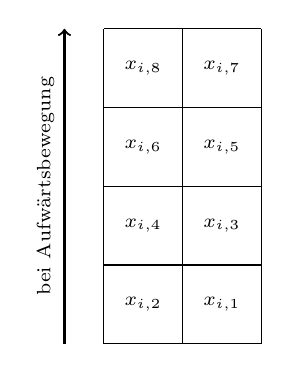
\begin{tikzpicture}[font=\scriptsize]
    \draw[step=1cm] (0,0) grid (2,4);
    \foreach \i in {1,...,4} {
      \foreach \j [evaluate=\k using {int(2*(\i-1)+\j)}] in {1,2} {
        \node at (2.5 - \j, -.5 + \i) {$x_{i,\k}$};
      }
    }
    \draw[->,thick] (-.5, 0) -- node[above,sloped] {bei Aufwärtsbewegung} (-.5, 4);
  \end{tikzpicture}
  \qquad
  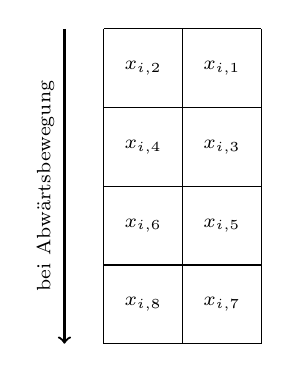
\begin{tikzpicture}[font=\scriptsize,yscale=-1]
    \draw[step=1cm] (0,0) grid (2,4);
    \foreach \i in {1,...,4} {
      \foreach \j [evaluate=\k using {int(2*(\i-1)+\j)}] in {1,2} {
        \node at (2.5 - \j, -.5 + \i) {$x_{i,\k}$};
      }
    }
    \draw[->,thick] (-.5, 0) -- node[above,sloped] {bei Abwärtsbewegung} (-.5, 4);
  \end{tikzpicture}
  \caption{Verteilung der finalen Datensequenz $x∈\GF(2^8)^{172}$ in $Q$. Links: $x_1, x_2,\dotsc$ werden schlangenförmig von unten beginnend in den noch nicht durch Positionsmuster o.\,ä.\ belegten Platz verteilt, wobei jeweils zwei Spalten gemeinsam verwendet werden. Mitte und rechts: Verteilung der $8$ Bits des $i$-ten Bytes $x_i$ bei Auf- und Abwärtsbewegung der eben beschriebenen Schlangenlinien.}
  \label{fig:bitPlacement}
\end{figure}
Bei $172$ Bytes werden so insgesamt $172⋅8=1376$ Einträge von $Q$ belegt, so dass von den $1383$ Pixeln im Datenbereich am Ende $7$ unbelegt (weiß) bleiben.

\subsection{Maske und Format-Information}
Nach Platzierung von $x$ in der Matrix $Q$ können durch Zufall Muster auftreten, die den Positions-Mustern ähneln und so die Bilderkennung erschweren. Um dies zu verhindern, wird eine von acht \emph{Muster-Matrizen} $M^0,\dotsc, M^7 ∈ \GF(2)^{41×41}$ ausgewählt und auf $Q$ addiert. Dabei wird nur der Datenbereich von $Q$ verändert: $M^k_{i,j}=1$ kann nur gelten, vonn $Q_{i,j}$ nicht zu einem Auffindungs-Muster oder der Format-Information gehört. Beim Lesen des QR-Codes wird dieser Schritt wieder rückgängig gemacht, indem das entsprechende $M^k$ nochmal auf die Summe $Q+M^k$ addiert wird, denn $Q+M^k+M^k = Q$.

Am Ende wird das verwendete Fehlerlevel (bei uns: M) und die Nummer der verwendeten Maske $k∈\{0,\dotsc,7\}$ zu einem binären 5-Tupel 
$f$ zusammengefasst, \zB $f = \underbrace{00}_{\text{M}} \underbrace{101}_{\op{bin}_3{k}}$ und mit einem $(15,5)$-Code $\hat\C$ mit Minimaldistanz $\d(\hat\C)=7$ zu einer 15-Bit-Nachricht $φ = E_{\hat\C}(f)$ codiert. Darauf wird schließlich noch die Folge $γ=101010000010010$ addiert; dadurch erreicht man, dass die finale Format-Information $ϑ=φ+γ$ nie der Nullvektor ist (in diesem Fall wäre er schwer vom Trenner um die Positionsmuster zu unterscheiden). Schließlich wird $ϑ$ \emph{zweimal} in die Bereiche um die Positionsmuster geschrieben. Diese Information, ohne die keine Decodierung des QR-Codes möglich ist, ist also besonders gut gesichert.

\subsection{Decodierung}
Zur Decodierung werden alle genannten Schritte in umgekehrter Reihenfolge durchgeführt: Nachdem ein Bilderkennungs-Algorithmus den QR-Code aufgefunden und gedreht bzw.\ entzerrt hat, wird zunächst die Format- und Maskeninformation ausgelesen, die Maske rückgängig gemacht, die vier Codewörter extrahiert, jedes davon mit einem Reed-Solomon-Decodieralgorithmus (den wir hier nicht behandelt haben) decodiert, woraus sich die Nachricht $m(w)$ ergibt. Anhand von Modus-Indikator $0010$ und Zeichenzähler kann schließlich die Originalnachricht rekonstruiert werden, solange in jedem der vier Codewörter höchstens $8$ Lesefehler vorliegen.
\begin{Center}
  \qrcode*{Wir hoffen, dass Ihnen die Vorlesung gefallen hat, und wünschen viel Erfolg bei der Prüfungsvorbereitung!}
\end{Center}